\documentclass[12pt]{article}
\usepackage[italian]{babel}
\usepackage{graphicx}
\usepackage[section]{placeins}
\usepackage{amsmath}% http://ctan.org/pkg/amsmath
\usepackage{enumitem}
\usepackage{graphicx}
\usepackage[section]{placeins}

\title{Elaborazione delle Immagini}
\author{Giuseppe Facchi}
\date{A.A. 2020-2021}

\begin{document}
\maketitle
\newpage
\tableofcontents
\newpage

\section{Introduzione}
\subsection{Radiometria e Fotometria}
\subsection{Radiometria}

Considera la luce come una radiazione elettromagnetica (em).
\\ \textbf{Studia le radiazioni em} e il \textbf{trasferimento di energia radiante} tramite un \textit{insieme di grandezze fisiche scalari funzioni della lunghezza d'onda}
\paragraph{Misure Radiometriche}
\begin{itemize}
    \item \textbf{Energia Totale Q}
    \item Flusso Raggiante F
    \item Irraggiamento
    \item Intensità Radiante
    \item Radianza
\end{itemize}
$$E(\lambda)R(\lambda)=Colore$$
Dove:
\begin{itemize}[label=]
    \item $E(\lambda)$: \textit{Distribuzione spettrale di energia} (Funzione della \textbf{lunghezza d'onda})
    \item $R(\lambda)$: \textit{Percentuale di luce riflessa} (Funzione della \textbf{lunghezza d'onda})
\end{itemize}
\subsection{Fotometria}
\textbf{Studia come le radiazioni em vengono percepite dall'uomo} mediante la valutazione \textbf{visiva} di uno stimolo radiometrico
\paragraph{Efficacia Luminosa Spettrale $V(\lambda)$}
\subsection{Adattamento del sistema visivo umano alle condizioni ambientali}
La gamma di luminosità a cui l'occhio può adattarsi è enorme. L'occhio non funziona \textbf{simultaneamente} sull'intera gamma di livelli di colre, utilizza quindi un \textbf{meccanismo di adattamento}.
\paragraph{Legge di Weber}
Nella visione dato uno \textbf{stimolo d'intensità} $I$ per cogliere uno stimolo d'intensità superiore occorre una certa soglia $\Delta I$, dove $${\Delta I \over I }=C$$
L'unità di misura dello stimolo è la differenza dello stimolo appena distinguibile (JND). La legge di Weber è \textbf{empirica} e tende a non valore in condizioni di oscurità o elevata luminosità
\newpage
\section{Digitalizzazione}
\subsection{Introduzione}
Esistono tre tipi di immagini
\begin{itemize}
    \item Binarie
    \item Livelli di Grigio
    \item A Colori
\end{itemize}
\paragraph{Immagine Digitale} Immagine 2D $I(r,c)$ rappresentata da una matrice discreta di campioni
\\[12pt]Per convertire un'immagine da \textbf{analogica} a \textbf{digitale}:
\begin{itemize}
    \item \textbf{Campionamento Spaziale} (operazione di digitalizzazione dei valori delle \textbf{coordinate}): \textit{Si prendono un numero finito di punti nel dominio spaziale}
    \item \textbf{Quantizzazione} (operazione di digitalizzazione dei valori di \textbf{ampiezza}): \textit{Si prendono un numero finito di valori nel range $f(x,y)$}
\end{itemize}
Nella formazione dell'immagine intervengono:
\begin{itemize}
    \item Parametri Geometrici
    \item Parametri Ottici
    \item Parametri Fotometrici
    \item Parametri del Sensore
\end{itemize}
$$Intensita` = Illuminazione \times Riflettanza$$
$$Irradianza = i(x,y) \times r(x,y)$$
\begin{itemize}
    \item L'\textbf{illuminazione} dà luogo a variazioni \textbf{lente}
    \item La \textbf{riflettanza} dà luogo a variazioni \textbf{brusche}
\end{itemize}
\subsection{Risoluzione}
\paragraph{Livelli di Grigio} La più piccola differenza del livello di grigio che riusciamo a discriminare
\\[12pt]
La risoluzione è un concetto relativo a diversi fattori ad esempio risoluzione del sensore, risoluzione dell'apparecchiatura di resa eccetera
\paragraph{Range Dinamico} Rapporto tra l'intensità massima misurabile e il liverro minimo di intensità rilevabile nel sistema. Il \textbf{limite massimo} è chiamato \textbf{saturazione}. Il \textbf{limite minimo} è chiamato \textbf{rumore}.
\newpage
\section{Pre-Elaborazione delle Immagini}
\subsection{Enhancement}
\section{Operatori Puntuali}
L'intorno del pixel è spesso chiamato \textbf{finestra} o \textbf{filtro}
\subsection{Operazioni puntuali omogenee} Il risultato dipende solo dal valore del pixel in cui è applicata
\begin{itemize}
    \item Somma o differenza di una costante a tutti i pixel
    \item Inversione della scala dei grigi
    \item Clipping
    \item Modifiche del contrasto
    \item Equalizzazione dell'istogramma
    \item Presentazione falso in colore
\end{itemize}

\begin{figure}[!htb]
    \centering
    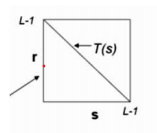
\includegraphics[width=0.3\textwidth]{Images/rsT.png}
    \caption{Trasformazione r = T(s)}
\end{figure}

\subsubsection{Trasformazione dei livelli di grigio}
Utilizzo della \textbf{LUT}: una tabella con tante entry quante sono i possibili valori di ingresso all’operazione. \textbf{Ogni entry della LUT contiene il valore (precalcolato) della trasformazione corrispondente al valore di grigio che fa da indice}. Quindi il calcolo si riduce alla \textbf{sostituzione di un valore di grigio con l’elemento della tabella} che ha come indice quel valore di grigio.
\subsubsection{Istogramma}
Rappresentato come $H(k)$, numero di pixel con livello di grigio corrispondente a $k$
\begin{figure}[!htb]
    \centering
    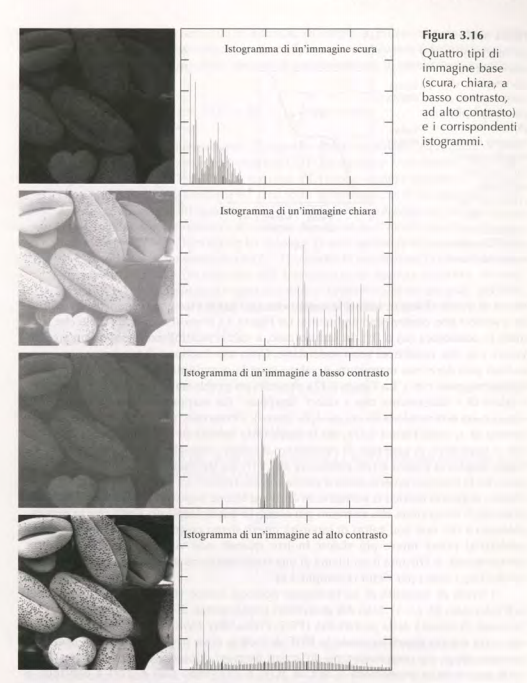
\includegraphics[width=0.7\textwidth]{Images/hist.png}
    \caption{Trasformazione r = T(s)}
\end{figure}
\FloatBarrier
\subsubsection{Istogramma normalizzato}
Rappresenta la frequenza di occupazione dei livelli (stima di probabilità di avere il valore $k$)
\subsubsection{Operatore di thresholding (binarizzazione)}
\subsubsection{Operazione di clipping}
I valori estremi vengono saturati
\subsubsection{Operazione di stretching}
Migliora il contrasto dell'immagine espandendo la dinamica dei livelli di grigio su un intervallo più ampio
\newpage
\subsection{Operazioni puntuali non omogenee}
\subsubsection{Scaling Logartmico}
\begin{figure}[!htb]
    \centering
    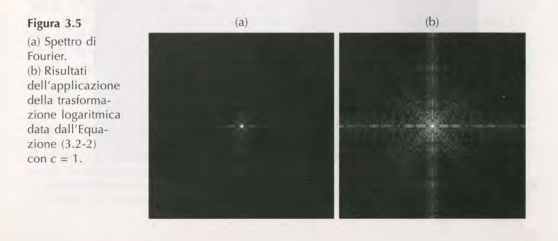
\includegraphics[width=1\textwidth]{Images/log.png}
    \caption{Trasformazione Logaritmica}
\end{figure}
\FloatBarrier
\begin{itemize}
    \item \textbf{Compressione} della dinamica per \textbf{alti valori} di $r$
    \item \textbf{Espansione} della dinamica per \textbf{bassi valori} di $r$
\end{itemize}
\subsubsection{Gamma Correction}
\begin{itemize}
    \item \textbf{Espansione} della dinamica per \textbf{alti valori} di $r$
    \item \textbf{Compressione} della dinamica per \textbf{bassi valori} di $r$
    \item Richiede normalizzazione in range 0:255
\end{itemize}
\FloatBarrier
\begin{figure}[!htb]
    \centering
    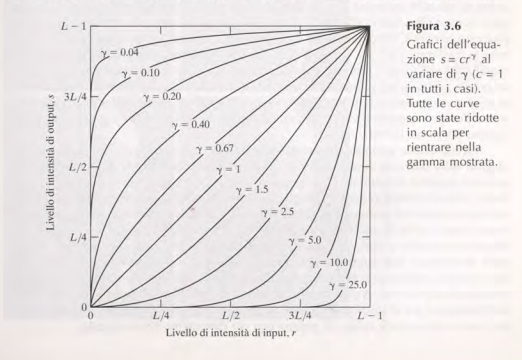
\includegraphics[width=0.6\textwidth]{Images/gamma.png}
    \caption{Gamma Correction}
\end{figure}
\FloatBarrier
\begin{figure}[!htb]
    \centering
    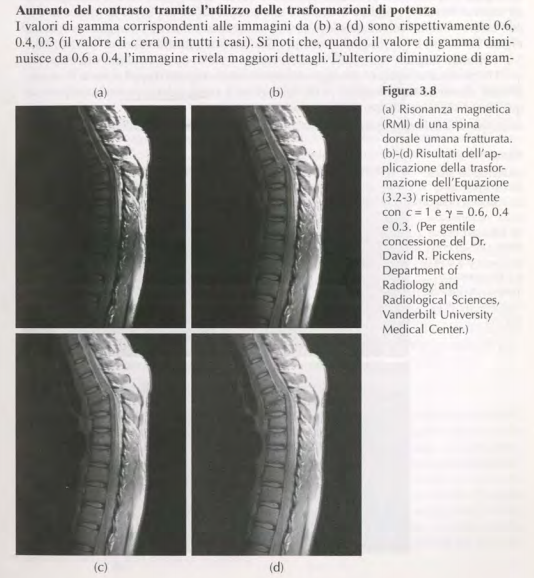
\includegraphics[width=0.7\textwidth]{Images/gamma3.png}
    \caption{Gamma Correction}
\end{figure}
\FloatBarrier
\subsubsection{Modifiche del contrasto}
\begin{itemize}
    \item Se la pendenza della curva di mapping è minore di 45° si parla di \textbf{compressione} del contrasto
    \item Se la pendenza della curva di mapping è maggiore di 45° si parla di \textbf{espansione} del contrasto
\end{itemize}
\begin{figure}[!htb]
    \centering
    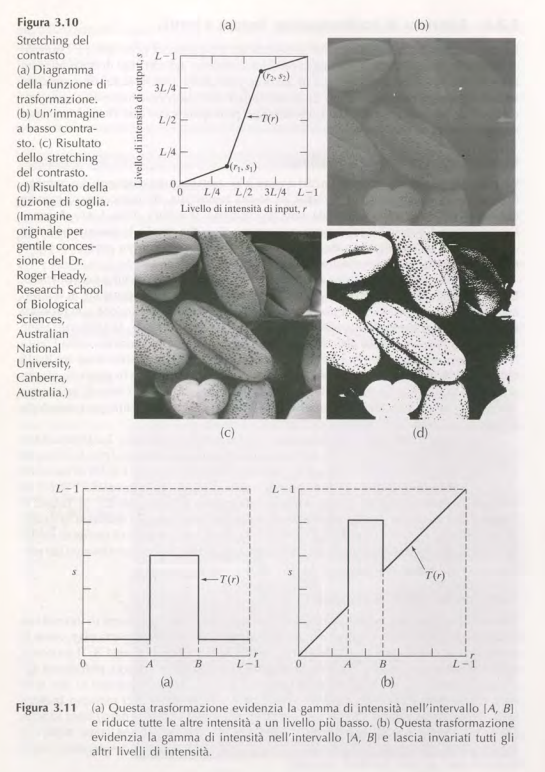
\includegraphics[width=0.7\textwidth]{Images/contrasto.png}
    \caption{Stretching del contrasto}
\end{figure}
\FloatBarrier
\subsubsection{Selezione a piani di bit}
\begin{figure}[!htb]
    \centering
    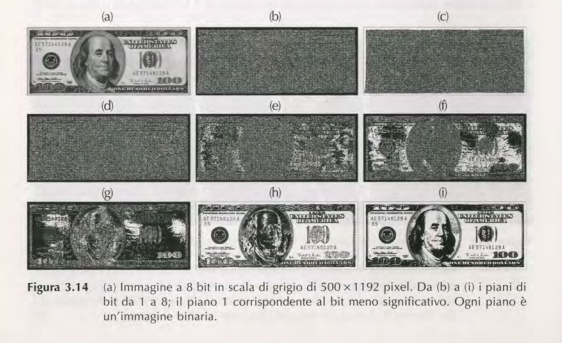
\includegraphics[width=0.7\textwidth]{Images/8b.png}
    \caption{Selezione a piani di bit}
\end{figure}
\FloatBarrier
\subsubsection{Slicing}
Per un certo intervallo di grigio viene impostato un livello $L$
\subsubsection{Equalizzazione dell'istogramma}
Sfrutta il concetto alla base del contrast stretching. Muta la forma dell'istogramma per bilanciare meglio i livelli. Ne deriva un incremento della gamma dinamica dei pixel.\\ L'equalizzazione non sempre migliora la qualità
\begin{itemize}
    \item Non tiene conto delle caratteristiche locali dell'immagine
    \item Per immagini che hanno un istogramma "quasi binario" o a basso contrasto si possono creare falsi contorni
    \item Può esaltare il rumore e sgranare
\end{itemize}
L'immagine per una buona equalizzazione deve essere:
\begin{itemize}
    \item Sovraesposta/Sottoesposta
    \item Se non lo è si attua un'\textbf{equalizzazione locale}
\end{itemize}
\begin{figure}[!htb]
    \centering
    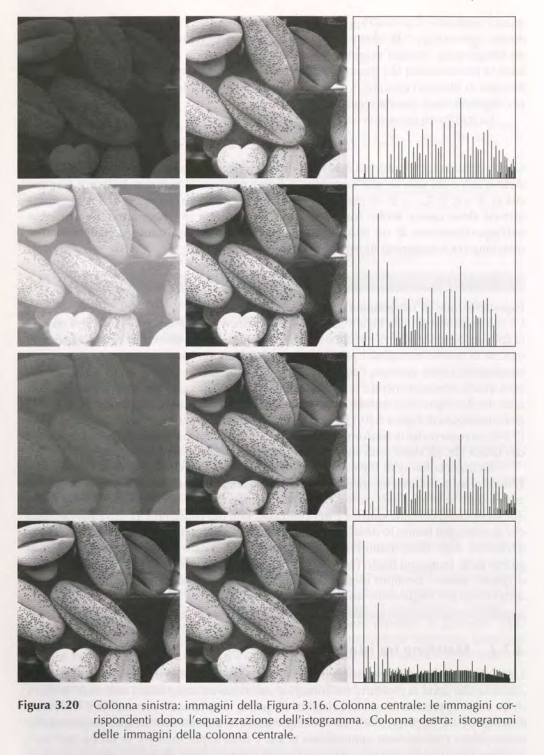
\includegraphics[width=0.7\textwidth]{Images/histeq.png}
    \caption{Equalizzazione dell'istogramma}
\end{figure}
\FloatBarrier
\subsubsection{Media Varianza e Deviazione Standard}
\subsubsection{Correzione puntuale dell'illuminazione}
L'illuminazione della scena può non essere \textbf{uniforme}. Se la \textbf{degradazione} dell'immagine è di natura sistemica possiamo procedere come segue
$$f(i,j)=e(i,j)g(i,j)$$
Dove:
\begin{itemize}[label=]
    \item $f(i,j)$: \textit{Immagine degradata}
    \item $e(i,j)$: \textit{Cambiamento rispetto al sistema ideale} (può essere costante)
    \item $g(i,j)$: \textit{Immagine ideale}
\end{itemize}
\newpage
\section{Operatori Locali}
\subsection{Restauro}
Il processo di restauro può essere modellato come una funzione di degrado $H$ che unitamente ad un rumore additivo, agisce sull'immagine di ingresso $f(x,y)$ nel produrre l'immagine degradata $g(x,y)$.
\\Data $g(x,y)$ e una certa conoscenza della funzione di degrado $H$ e del termine di rumore additivo l'obiettivo del restauro è di \textbf{ottenere la migliore stima possibile dell'immagine non degradata}
\paragraph{Tecniche}
\begin{itemize}
    \item \textbf{Tecniche del dominio spaziale} (usate quando c'è rumore additivo)
    \item \textbf{Tecniche nel dominio della frequenza}
\end{itemize}
\subsection{Filtri spaziali}
Caratterizzato da un \textbf{intorno} e un'\textbf{operazione che deve essere eseguita sui pixel dell'immagine in quell'intorno}.\\
Il processo di filtraggio genera una nuova immagine spostando il filtro lungo tutta l'immagine.\\
Se l'operazione eseguita è lineare parliamo di \textbf{filtri spaziali lineari}. Altrimenti parliamo di \textbf{filtri non lineari}.\\
Comportamento nelle zone periferiche dell’immagine (contorno)
\begin{itemize}
    \item Si aggiungono dei pixel sui contorni a valore costante (neri, grigi,...)
    \item Si duplicano i pixel terminali
    \item Si usano nei calcoli solo i pixel dell’immagine compresi nella maschera
    \item Si considera l’immagine avvolta su un toro
    \item Si riduce l’area dell’immagine (nessuna aggiunta di informazione)
\end{itemize}

\subsubsection{Regressione}
\subsubsection{Convoluzione}
\subsubsection{Smoothing}
Effettuare uno smoothing significa letteralmente “appianare” , “levigare” una superficie. Quando applichiamo un filtro di smoothing ad un’immagine otteniamo, da un lato la possibilità di ridurre il rumore, dall’altro il rischio di creare un blurring (“sfocatura”) più o meno indesiderato a seconda dello scopo dell’immagine da processare
\newpage
\subsubsection{Media Artimetica}
Il livello di grigio del pixel centrale corrisponde alla media aritmetica dei
valori dei pixel compresi nell’intorno
\begin{figure}[!htb]
    \centering
    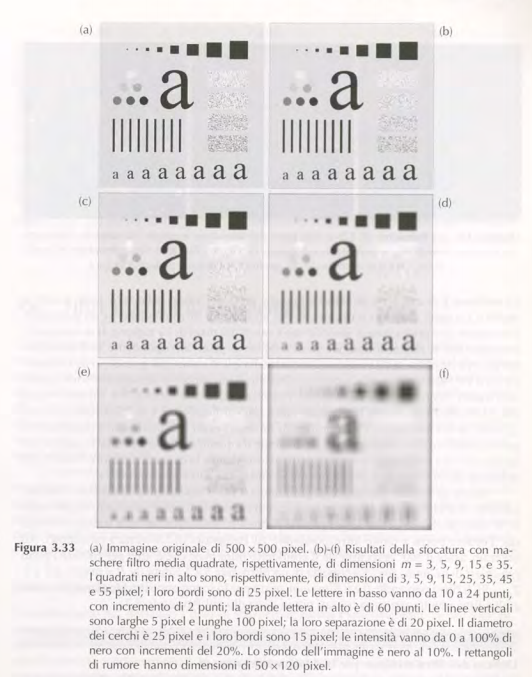
\includegraphics[width=0.7\textwidth]{Images/media.png}
    \caption{Filtro di media}
\end{figure}
\FloatBarrier
\begin{figure}[!htb]
    \centering
    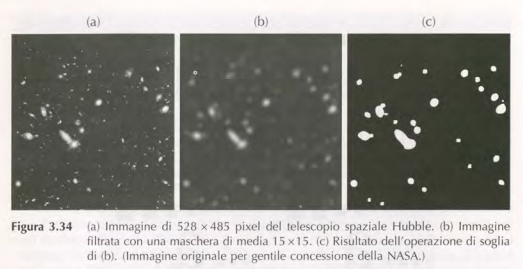
\includegraphics[width=0.7\textwidth]{Images/mediasoglia.png}
    \caption{Filtro di media con soglia}
\end{figure}
\FloatBarrier
\subsubsection{Filtraggio gaussiano}
I filtri di smoothing sono usati per il blurring dell’immagine e per la riduzione del rumore.
\\\textbf{L’operazione di blurring è normalmente utilizzata in fase di preelaborazione, allo scopo di eliminare piccoli dettagli}
Vantaggi:
\begin{itemize}
    \item efficace sul rumore di tipo guassiano
    \item facile da implementare ed ottimizzare (è lineare)
\end{itemize}

Svantaggi:
\begin{itemize}
    \item Si alterano anche i contorni
    \item Diffonde il rumore sale e pepe
\end{itemize}

Lo sfuocamento puo’ essere un vantaggio (elimina i dettagli) o uno svantaggio (sfuca i contorni degli oggetti significativi) a seconda dell'applicazione.
Aumentando la dimensione della finestra aumenta lo sfuocamento della immagine, ma non necessariamente si elimina il rumore impulsivo (salt-and-pepper).
\subsubsection{Filtraggio Mediano}
Forzare i pixel ad assumere un valore uguale a quello di uno dei pixel circostanti, eliminando così eventuali picchi isolati di intensità. Elimina molto bene gli eventuali pixel isolati che solitamente corrispondono al rumore di tipo impulsivo.
Anche il fitro mediano può usare diverse maschere. Queste devono essere di
dimensioni dispari e simmetriche rispetto all’origine. I problemi sui bordi dell’immagine di gestiscono nei modi citati precedentemente. \\
\begin{figure}[!htb]
    \centering
    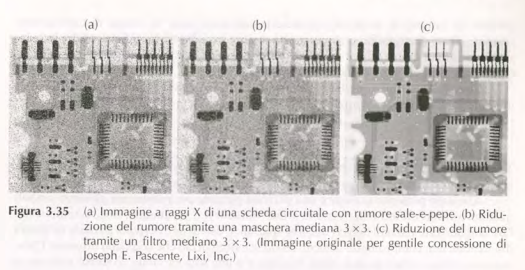
\includegraphics[width=0.7\textwidth]{Images/mediano.png}
    \caption{Filtro mediano}
\end{figure}
\FloatBarrier
\newpage
\section{Operatori Locali EDGE}
\subsection{Bande di Mach}
Bande di livello di grigio costante, vengono percepite non uniformi
\subsection{Sharpening}
I contorni, o edge, sono cambiamenti significativi e locali all’interno di un’immagine. Tipicamente si verificano in prossimità dei bordi di diverse regioni dell’immagine. Gli edge trovati non corrispondono necessariamente ai contorni di oggetti reali. Gli edge sono punti dell’immagine dove si e’ verificata una alta variazione dei valori di intensità luminosa.
\begin{itemize}
    \item \textbf{Complementari ai filtri di smoothing}, i filtri di sharpening sono utilizzati per aumentare il contrasto locale dell’immagine, in modo da arricchire i dettagli fini ed evidenziare i contorni degli oggetti.
    \item Possono provocare l’\textbf{aumento del rumore} presente nell’immagine.
\end{itemize}
La derivata prima è diversa da 0 lungo tutta la rampa, mentre la derivata seconda è diversa da 0 solo all’inizio e alla fine della rampa. Poiché i contorni nelle immagini digitali sono generalmente rampe, si può concludere che la derivata prima produce edge piuttosto spessi, mentre la derivata seconda dà luogo a edge più sottili ma “doppi”.\\
\textbf{La somma dei pesi delle maschere e’ zero. Risposta nulla su regioni di livello di grigio costante}
\subsubsection{Derivate seconde - Laplaciano}
La risposta è indipendente dalla direzione delle discontinuità dell'immagine a cui il filtro è applicato. Dato che le derivate sono operazioni lineari, l'equazione laplaciana è un operatore lineare.\\
Dato che l'equazione laplaciana è un operatore derivativo, il suo utilizzo mette in evidenza le discontinuità di intensità di un'immagine e pone in secondo piano le regioni con livelli di intensità che variano lentamente. Ciò tende a produrre immagini con linee grigiastre e altre discontinuità, su uno sfondo scuro e anonimo.\\
Le caratteristiche dello sfondo possono essere "recuperate", mantenendo lo
sharpening dell 'immagine dato dal metodo laplaciano, e aggiungendo l'immagine laplaciana all'originale.
\begin{figure}[!htb]
    \centering
    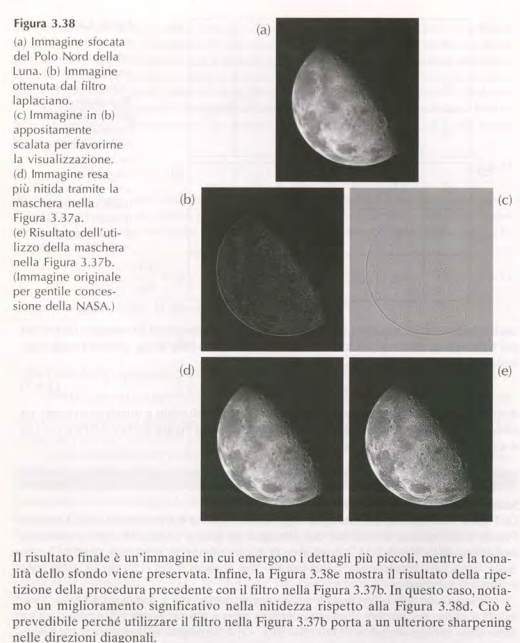
\includegraphics[width=0.7\textwidth]{Images/lap.png}
    \caption{Filtro Laplaciano}
\end{figure}
\FloatBarrier

\subsubsection{Unsharp masking - high-boost filtering}
IUn tipico processo utilizzato dall'industria grafica e pubblicitaria per dare sharpening all'immagine consiste nel sottrarre una versione sfocata (unsharp) dell'immagine dall'originale.
\\Il procedimento di unsharp masking si puo’ implementare in due passi:
\begin{enumerate}
    \item Sottrarre all’immagine originaria una versione “smooth” della stessa
    \item Sommare l’immagine risultante all’immagine originaria
    \item Aggiungere la maschera all'originale
\end{enumerate}
\begin{figure}[!htb]
    \centering
    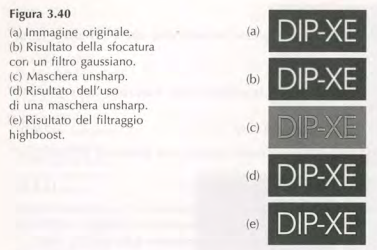
\includegraphics[width=0.7\textwidth]{Images/highboost.png}
    \caption{High-boost filtering}
\end{figure}
\FloatBarrier
\subsubsection{Derivate prime - Gradiente}
Il gradiente di un'immagine è un \textbf{campo vettoriale}. Ogni vettore del campo punta nella direzione in cui localmente l'immagine presenta il maggior incremento d'intensità e ha una lunghezza che rappresenta il tasso di variazione. Il vettore gradiente può essere rappresentato in coordinate polari.
\\\textit{Lunghezza ed angolo sono ottenute come funzione delle derivate dell'immagine}
\begin{figure}[!htb]
    \centering
    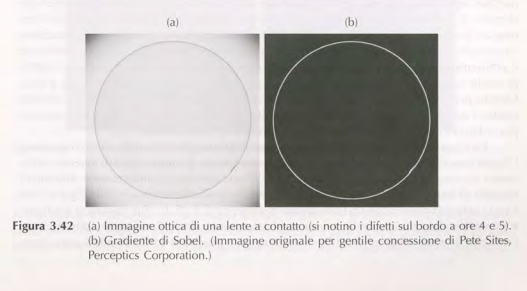
\includegraphics[width=0.7\textwidth]{Images/grad.png}
    \caption{Immagine Gradiente}
\end{figure}
\FloatBarrier
\subsection{Contorni}
Il rumore influenza l’identificazione di un contorno.
\begin{itemize}
    \item Al crescere del rumore derivata prima e seconda diventano sempre meno riconoscibili
    \item La derivata seconda è più sensibile al rumore
    \item L’effetto del rumore non impedisce di riconoscere il contorno nell’immagine, ma rende via via sempre meno interpretabili le corrispondenti derivate.
\end{itemize}
\newpage
\section{Operatori Geometrici}
Le operazioni spaziali sono eseguite direttamente sui pixel di una data immagine. Le classifichiamo in tre categorie:
\begin{itemize}
    \item operazioni a singolo pixel
    \item operazioni basate sull'intorno
    \item trasformazioni spaziali geometriche
\end{itemize}

\subsection{Operazioni a singolo pixel}
La più semplice operazione che possiamo eseguire su un'immagine digitale è quella di alterarne il valore dei pixel basandoci sulla loro intensità. Ad esempio il \textbf{negativo}
\subsection{Operazioni basate sull'intorno}
Denotiamo con $S_{xy}$ l'insieme delle coordinate di un intorno centrato su un punto arbitrario $(x, y)$ in un'immagine $f$. Le operazioni basate sull'intorno generano un pixel alle stesse coordinate nell'immagine di output, $g$, il cui valore è determinato da una specifica operazione che coinvolge i pixel nell'immagine di input le cui coordinate stanno in $S_{xy}$. Per esempio, supponiamo che l'operazione consista nel calcolare la media dei valori dei pixel in un intorno rettangolare di dimensioni $m \times n$ centrato in $(x, y)$.
\subsection{Trasformazioni spaziali geometriche e registrazione di immagini}
Le trasformazioni geometriche modificano le relazioni spaziali tra i pixel di un'immagine. Queste trasformazioni vengono spesso chiamate rubber-sheet (letteralmente "foglio di plastica") dato che possono essere associate al processo di stampa di un'immagine su un foglio di plastica, sul quale si eseguono poi delle deformazioni opportune.\\
Una trasformazione geometrica consiste di due distinte operazioni
\begin{itemize}
    \item una trasformazione spaziale delle coordinate
    \item un'interpolazione delle intensità che assegna i giusti valori ai pixel dopo la trasformazione
\end{itemize}
\begin{figure}[!htb]
    \centering
    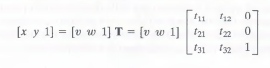
\includegraphics[width=0.3\textwidth]{Images/trasfaff.png}
    \caption{Trasformazione Affine}
\end{figure}
\FloatBarrier
\begin{figure}[!htb]
    \centering
    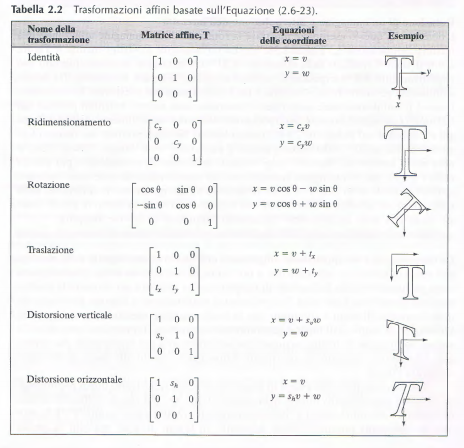
\includegraphics[width=0.7\textwidth]{Images/affini.png}
    \caption{Valori matrice affine}
\end{figure}
\FloatBarrier
Il primo, detto \textbf{forward mapping} (letteralmente "assegnamento in avanti"), consiste nel visitare i pixel dell'immagine di input e per ciascuna posizione (v, w), calcolare la corrispondente posizione spaziale, (x, y), del pixel nell'immagine di output utilizzando, direttamente l'Equazione di Trasformazione Affine. Potrebbe però accadere che due o più pixel dell'immagine di input siano assegnati alla stessa posizione spaziale nell'immagine di output, ponendo quindi il problema dell'individuazione di un unico valore di output. Inoltre è possibile che qualche posizione nell'immagine di output non venga per nulla considerata.\\ Il secondo approccio detto \textbf{inverse mapping} (letteralmente "assegnamento inverso") visita le posizioni spaziali dei pixel di output e per ciascuna di esse calcola le corrispondenti coordinate nell'immagine di input utilizzando $(v, w) = T^{-1}(x, y)$. Viene quindi calcolato il valore di intensità da assegnare al pixel utilizzando una tecnica di interpolazione considerando i pixel di input più vicini. L'inverse mapping può essere implementato in maniera più efficiente rispetto al forward mapping
\subsubsection{Zooming}
L'\textbf{interpolazione nearest neighbor} assegna a ogni nuova posizione l'intensità del pixel più prossimo nell'immagine originale. Questo approccio è molto semplice ma introduce artefatti, come distorsioni lungo gli edge, ed è quindi poco utilizzato nella pratica.\\
Un approccio più conveniente è l'\textbf{interpolazione bilineare}, con la quale si utilizzano i quattro pixel più vicini per stimare l'intensità da assegnare a ciascuna nuova posizione.\\
Il livello successivo di complessità è dato dall'\textbf{interpolazione bicubica}, che riguarda i sedici pixel più vicini al punto. Generalmente l'interpolazione bicubica preserva meglio i dettagli rispetto all'interpolazione bilineare.
\subsubsection{Rotazione}
\begin{figure}[!htb]
    \centering
    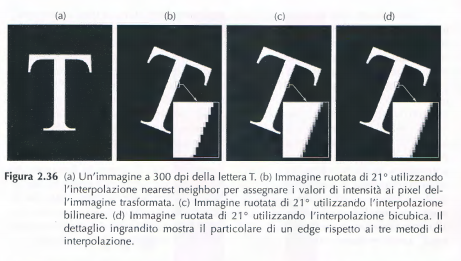
\includegraphics[width=0.7\textwidth]{Images/rot.png}
    \caption{Rotazione}
\end{figure}
\FloatBarrier
\subsubsection{Allineamento di due immagini}
Per risolvere tale problema si utilizzano i cosiddetti punti di controllo (detti anche "tie point", cioè punti corrispondenti), le cui posizioni sono note in entrambe le immagini di input e di riferimento. La selezione di tali punti può avvenire in maniera automatica o attraverso l'interazione con l'utente. In alcune applicazioni, i sistemi di imaging producono degli appositi artefatti utilizzando nei sensori delle alterazioni controllate (ottenute ad esempio mediante piccoli oggetti metallici). Ciò fa sì che le immagini catturate dal sistema presentino un insieme di punti noti (detti reseau mark) che possono essere usati come guide per determinare i punti di controllo. Il problema della stima di una funzione di trasformazione si risolve determinando i parametri del relativo modello.
\newpage
\section{Modelli del colore}
L'uso del termine primario è stato ampiamente frainteso nel senso che i
tre colori primari standard, mescolati in varie proporzioni di intensità, venivano considerati capaci di produrre tutti i colori visibili. \\
I colori primari possono essere mescolati per produrre i colori secondari -magenta (rosso e blu), ciano (verde e blu) e giallo (rosso e verde)-. Mescolare i tre colori primari o un colore secondario con il suo colore primario opposto, alle giuste intensità produce il bianco. \\
\begin{figure}[!htb]
    \centering
    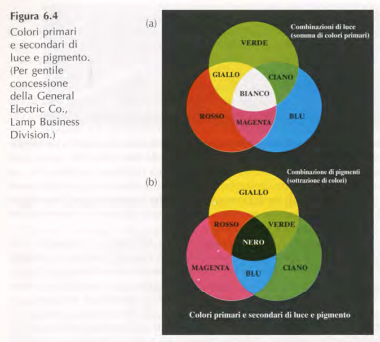
\includegraphics[width=0.7\textwidth]{Images/colori.png}
    \caption{Colori primari e secondari}
\end{figure}
\FloatBarrier
La differenziazione tra i colori primari della luce e i colori primari dei pigmenti (o coloranti) è importante. In questi, il colore primario è definito come un colore che sottrae o assorbe un colore primario di luce e riflette o trasmette gli altri due. Quindi, i colori primari dei pigmenti sono magenta, ciano e giallo e i colori secondari sono rosso, verde e blu. Questi colori vengono mostrati nella Figura. Una combinazione appropriata dei tre pigmenti primari o di un secondario con il suo primario opposto, produce il nero.\\

Scopo di un modello del colore è di consentirne la rappresentazione con
modalità standardizzate, che fanno normalmente riferimento ad un sistema di coordinate 3-D, o meglio ad un suo sotto-spazio, nel quale ogni colore è rappresentato da un punto.
\subsection{Modello RGB}
\begin{figure}[!htb]
    \centering
    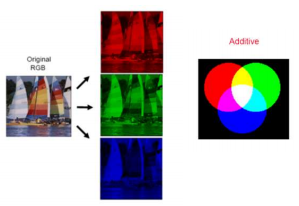
\includegraphics[width=0.5\textwidth]{Images/rgb.png}
    \caption{Modello RGB}
\end{figure}
\FloatBarrier
\subsection{Modello CMY}
\begin{figure}[!htb]
    \centering
    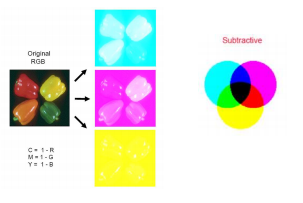
\includegraphics[width=0.5\textwidth]{Images/cmy.png}
    \caption{Modello CMY}
\end{figure}
\FloatBarrier
\newpage
\section{Trasformazioni di colore}
I valori dei pixel, in questo caso, sono triplette o quartetti (cioè gruppi di tre o quattro valori) nello spazio colore scelto per rappresentare le immagini
\begin{figure}[!htb]
    \centering
    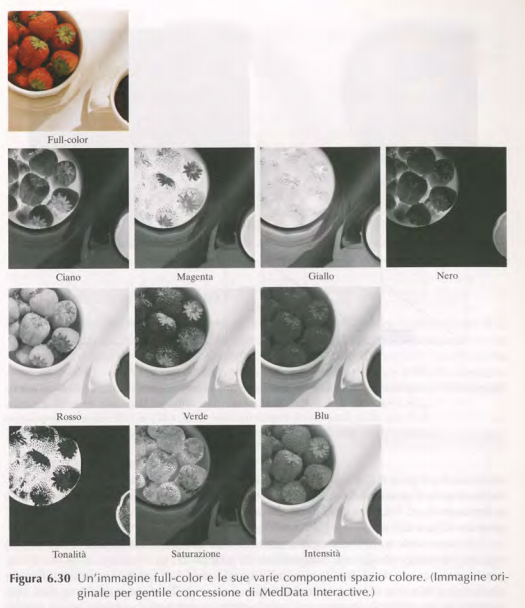
\includegraphics[width=0.8\textwidth]{Images/frag1.png}
    \caption{Modelli colore}
\end{figure}
\FloatBarrier
\begin{figure}[!htb]
    \centering
    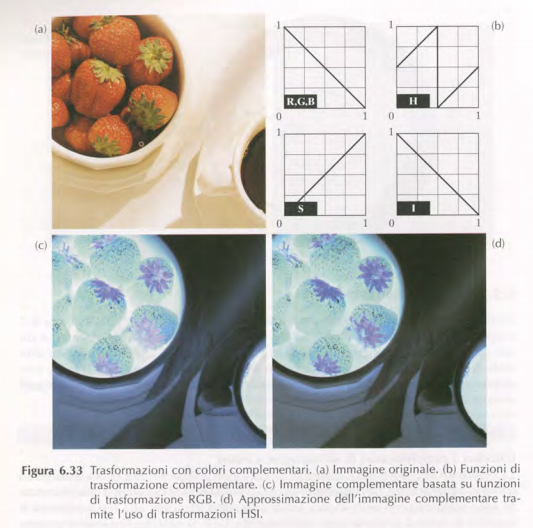
\includegraphics[width=0.8\textwidth]{Images/trasfcolori.png}
    \caption{Trasformazioni negative in spazi colore diversi}
\end{figure}
\FloatBarrier
\subsection{Operatori puntuali}
\subsubsection{Ripartizione di colore (slicing)}
Evidenziare una gamma specifica di colori in un'immagine è utile per separare gli oggetti
da ciò che li circonda. L'idea di base è
\begin{itemize}
    \item visualizzare i colori di interesse in modo tale che essi emergano dallo sfondo
    \item utilizzare la regione definita dai colori come maschera per ulteriori elaborazioni
\end{itemize}
Uno dei metodi più semplici per "ripartire" un'immagine a colori è trasformare i colori al di fuori della gamma di interesse in un colore neutrale non prominente
\begin{itemize}
    \item Cubo
    \item Sfera
\end{itemize}
Queste trasformazioni evidenziano i colori attorno al prototipo forzando tutti gli altri colori al punto medio dello spazio colore di riferimento (un punto neutrale scelto arbitrariamente). Per lo spazio RGB, ad esempio, un punto neutrale applicabile è il grigio medio (0.5, 0.5, 0.5)
\begin{figure}[!htb]
    \centering
    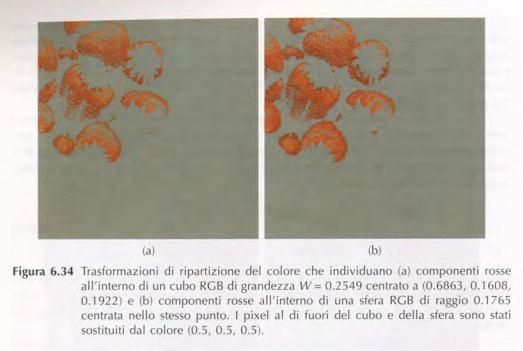
\includegraphics[width=0.8\textwidth]{Images/rip.png}
    \caption{Slicing colore}
\end{figure}
\FloatBarrier
\subsubsection{Trasformazioni di tonalità}
L'obiettivo è quello di regolare in maniera sperimentale la luminosità e il contrasto di un'immagine per dare la quantità di dettaglio massima su una gamma di intensità opportuna. Negli spazi RGB e CMY(K), questo significa trasformare tutte e tre (o quattro) componenti di colore con la stessa funzione
di trasformazione; nello spazio a colori HSI viene modificata solo la componente di intensità.
\begin{figure}[!htb]
    \centering
    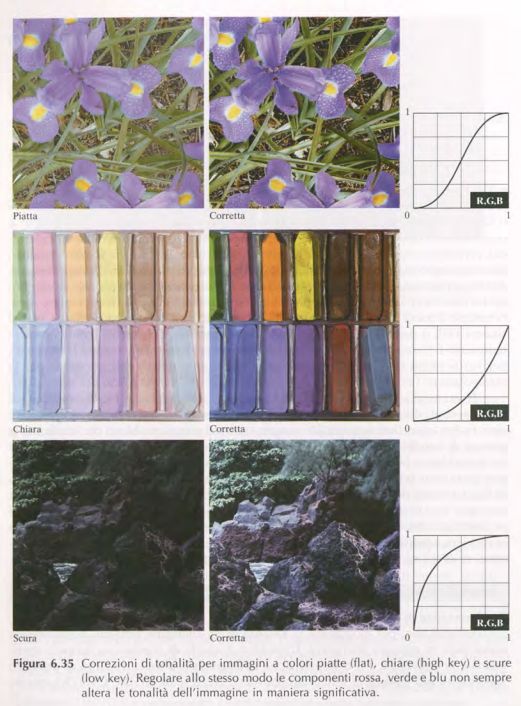
\includegraphics[width=0.8\textwidth]{Images/tonal.png}
    \caption{Slicing colore}
\end{figure}
\FloatBarrier
\subsubsection{Bilanciamento del colore}
La proporzione di ciascun colore può essere aumentata diminuendo la quantità del colore opposto (complementare) nell'immagine. In modo simile, essa può essere diminuita aumentando la proporzione dei due colori immediatamente adiacenti o diminuendo la percentuale dei due colori adiacenti al complementare. Supponiamo, ad esempio, che ci sia un'abbondanza di magenta in un'immagine RGB.
Esso può essere diminuito (1) rimuovendo del rosso e del blu o (2) aggiungendo del verde.
\begin{figure}[!htb]
    \centering
    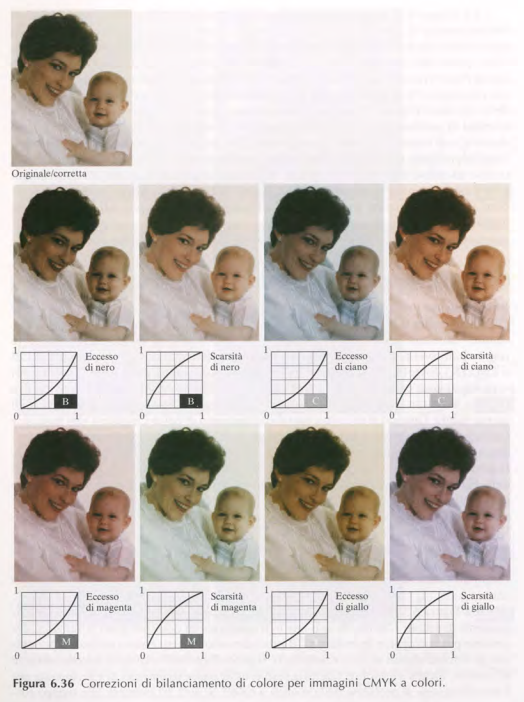
\includegraphics[width=0.8\textwidth]{Images/bil.png}
    \caption{Bilanciamento del colore}
\end{figure}
\FloatBarrier
\newpage
\subsubsection{Istogrammi}
Come prevedibile, di solito è difficile per un istogramma equalizzare le componenti di un'immagine a colori indipendentemente. Ciò porta a degli errori nel ominio del colore. Un metodo più logico è distribuire uniformemente le intensità del colore, lasciando i colori stessi (cioè le tonalità) invariati. Il seguente esempio mostra che lo spazio HSI è l'ideale per questo tipo di approccio.
\begin{figure}[!htb]
    \centering
    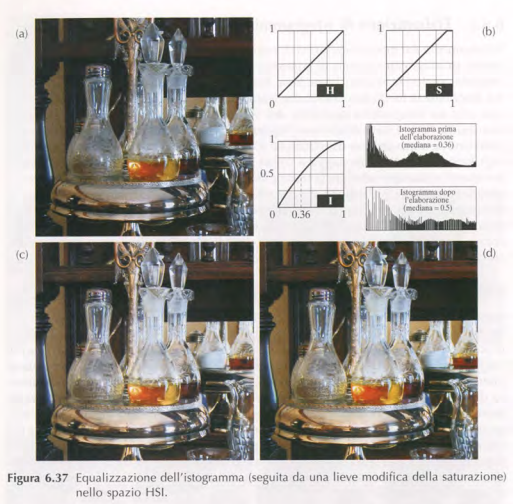
\includegraphics[width=0.8\textwidth]{Images/istcol.png}
    \caption{Istogramma immagine a colori}
\end{figure}
\FloatBarrier
\subsection{Operatori locali}
\subsubsection{Smoothing}
Applicare filtro di media su ogni componente RGB = Applicare filtro di media su I di HSI
\begin{figure}[!htb]
    \centering
    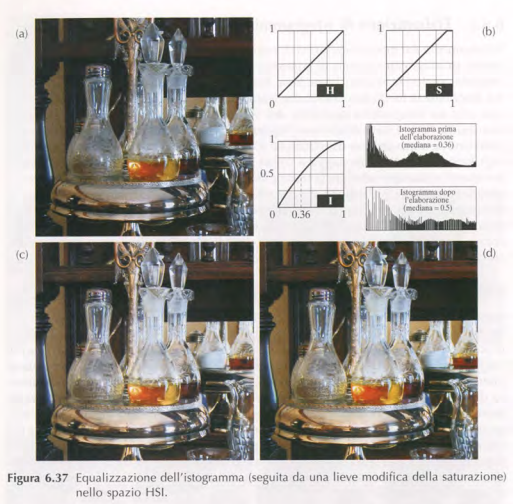
\includegraphics[width=0.8\textwidth]{Images/istcol.png}
    \caption{Filtro di Media}
\end{figure}
\FloatBarrier
\subsubsection{Sharpening}
Applicare filtro laplaciano (der. seconda) su ogni componente RGB = Applicare filtro laplaciano (der. seconda) su I di HSI
\begin{figure}[!htb]
    \centering
    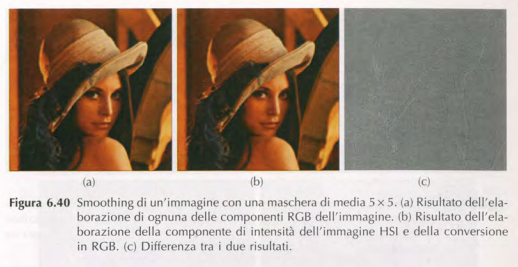
\includegraphics[width=0.8\textwidth]{Images/lapcol.png}
    \caption{Filtro Laplaciano}
\end{figure}
\FloatBarrier
\newpage
\section{Segmentazione immagini a colori}
Se si desidera segmentare un'immagine basandosi sul colore e, in aggiunta, si vuole portare avanti l'elaborazione su singoli piani, è naturale pensare subito allo spazio HSI perché il colore è ben rappresentato nell'immagine della tonalità.\\
Di solito, la saturazione è usata come immagine maschera per isolare ulteriori regioni di interesse rispetto alla tonalità. L'immagine dell'intensità è utilizzata meno di frequente per la segmentazione di
immagini a colori perché essa non contiene informazioni riguardanti i colori.
\subsection{Segmentazione in RGB}
L'approccio seguito è stato quello di calcolare il vettore medio $a$ utilizzando i punti colore contenuti all'interno del rettangolo nella Figura 6.44a e, poi, calcolare la deviazione standard dei valori rosso, verde e blu di quei campioni. È stata centrata una "scatola" su $a$ e le sue dimensioni lungo ognuno degli assi RGB sono state impostate come 1.25 volte la deviazione standard delle componenti rosse dei punti campione. Se denotiamo, ad esempio, con $\sigma_R$ la deviazione standard delle componenti rosse dei punti campione, le dimensioni della "scatola" lungo l'asse $R$ si estendono da ($a_R- 1.25\sigma_R$) ad ($a_R+ 1.25\sigma_R$), dove $a_R$ indica la componente rossa del vettore medio a. La Figura 6.44b mostra il risultato della codifica di ogni punto nell'intera immagine a colori come bianco, se esso non si trova sulla superficie o all'interno della scatola, e come nero altrimenti. Si noti come la regione segmentata è stata generalizzata secondo i campioni di colore racchiusi dal rettangolo.
\begin{figure}[!htb]
    \centering
    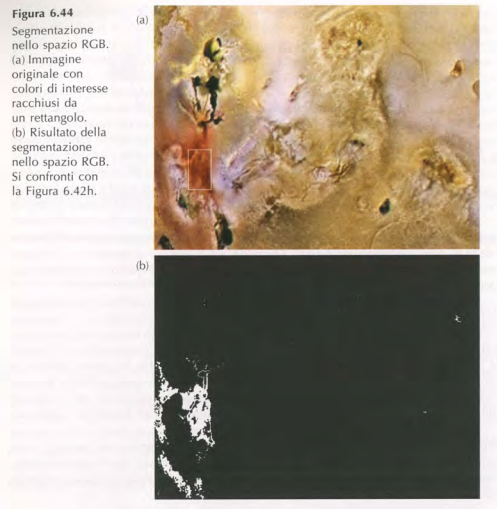
\includegraphics[width=0.8\textwidth]{Images/segcol.png}
    \caption{Segmentazione immagine a colori}
\end{figure}
\FloatBarrier
\subsection{Edge in RGB}
Sfortunatamente, il gradiente non è definito per quantità vettoriali. Quindi, sappiamo già in partenza che calcolare il gradiente sulle componenti RGB singole e, poi, usare il risultato per formare un'immagine a colori produce risultati non corretti (ma in certi casi accettabili). L’approccio piu’ semplice quindi prevede la somma delle magnitudini del gradiente per ciascun canale.
\begin{figure}[!htb]
    \centering
    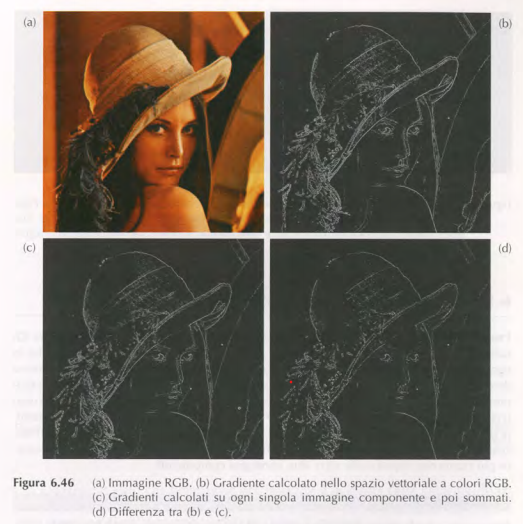
\includegraphics[width=0.8\textwidth]{Images/edgecol.png}
    \caption{Edge in RGB}
\end{figure}
\FloatBarrier
\begin{figure}[!htb]
    \centering
    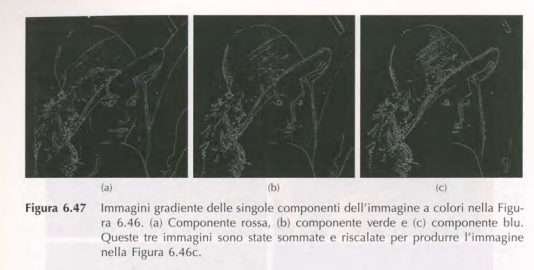
\includegraphics[width=0.8\textwidth]{Images/edgecol2.png}
    \caption{Edge in RGB}
\end{figure}
\FloatBarrier
\subsection{Rumore in RGB}
Di solito, il contenuto di rumore di un'immagine a colori ha le stesse caratteristiche in ogni canale, ma è anche possibile che i singoli canali vengano interessati in maniera diversa. È più probabile che livelli di rumore diversi siano causati da differenze nell'illuminazione disponibile per ogni singolo canale. Il filtraggio di immagini full-color può essere attuato sulle singole immagini componenti o direttamente nello spazio vettoriale a colori, in base al processo
\newpage
\section{Segmentazione di Immagini}
La segmentazione suddivide un'immagine nelle regioni o negli oggetti che la compongono. Il livello di dettaglio al quale viene effettuata la segmentazione dipende da ciò che si vuole ottenere. La segmentazione dovrebbe cioè arrestarsi quando gli oggetti o le regioni di interesse in una applicazione sono stati individuati. La maggior parte degli algoritmi di segmentazione presentati in questo capitolo si basa su una delle due proprietà di base dei valori di intensità: discontinuità e similarità.
\begin{itemize}
    \item Nel primo caso si tende a partizionare un'immagine basandosi sui bruschi cambiamenti di intensità, come ad esempio gli edge.
    \item  Nel secondo caso ci si basa sulle similarità tra regioni facendo riferimento a un insieme di criteri di similarità predefiniti.
\end{itemize}
Rientrano in quest'ultima tipologia le tecniche di soglia tura (thresholding), di crescita delle regioni
(region growing) e i metodi separa-e-fondi (split and merge).\\
Gli algoritmi di segmentazione per le immagini a toni di grigio si basano di solito
sulle proprietà di discontinuità e similarità dei valori di intensità. Nel primo caso, l'assunto è che i bordi delle regioni siano sufficientemente diversi l'uno dall'altro e dallo sfondo, in modo tale da permetterne l'individuazione basandosi sulla discontinuità delle intensità locali (segmentazione dipendente dagli edge). I metodi di segmentazione dipendenti dalla regione si basano, invece, sul partizionamento di un'immagine in regioni simili, tenendo conto di specifici criteri di similarità.
\begin{figure}[!htb]
    \centering
    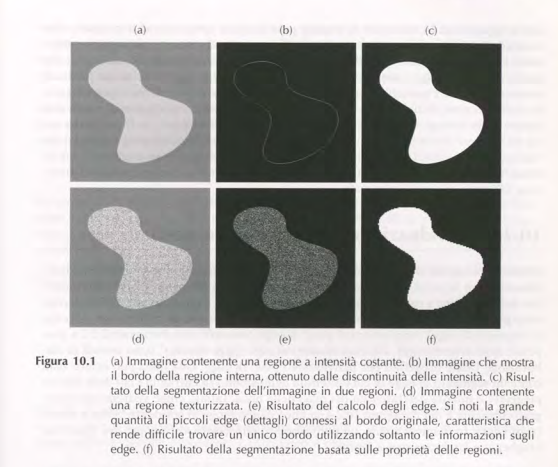
\includegraphics[width=0.8\textwidth]{Images/seg.png}
    \caption{Segmentazione}
\end{figure}
\FloatBarrier
Notiamo che (nella seconda riga) la regione più esterna è costante, così tutto quello che è necessario per risolvere questo problema di segmentazione è un predicato che differenzi le regioni costanti e quelle texturizzate. La deviazione standard dei valori dei pixel può essere usata a questo scopo, perché è diversa da zero nell'area interna (texture) zero altrove. La Figura 10.1f mostra il risultato della divisione dell'immagine originale in sottoregioni di dimensione 4 x 4. Ogni sottoregione è stata poi etichettata con bianco se la deviazione standard dei suoi pixel era positiva (cioè, se il predicato era
VERO) e zero altrimenti. Il risultato ha un aspetto "a blocchi" lungo il confine della regione perché i pixel all'interno di ciascun blocco 4 x 4 sono stati etichettati con lo stesso valore.
\newpage
\subsection{Edge detection}
Le derivate di primo ordine producono edge "spessi" e le derivate di secondo ordine edge più sottili. Una derivata seconda è molto più aggressiva della derivata prima nell'evidenziare i cambiamenti bruschi. Possiamo, quindi, aspettarci che le derivate seconde mettano in rilievo i dettagli più fini (incluso il rumore) molto meglio delle derivate prime. Il segno della derivata seconda può essere utilizzato per determinare il tipo di transizione di un edge. \\
Per calcolare le derivate prime e seconde in ogni pixel di una data immagine si utilizzano i filtri spaziali. Per la maschera filtro 3 x 3 nella Figura 10.3, la procedura è quella di calcolare la somma dei prodotti dei coefficienti della maschera con i valori di intensità nella regione inglobata dalla maschera.
\subsubsection{Individuazione Punti isolati}
L'individuazione di un punto si dovrebbe basare sulla derivata seconda, ciò implica l'uso del laplaciano. Diciamo che un punto è stato individuato nella posizione (x, y) su cui la maschera è centrata se il valore assoluto della risposta della maschera in quel punto supera uno specifico valore di soglia. Tali punti vengono denotati con 1 nell'immagine di output mentre tutti gli altri vengono posti a O, producendo, quindi, un 'immagine binaria'.
Si noti che, come è solito per una maschera derivativa, la somma dei coefficienti è zero, caratteristica che indica che la risposta della maschera sarà nulla nelle aree a intensità costante.
\begin{figure}[!htb]
    \centering
    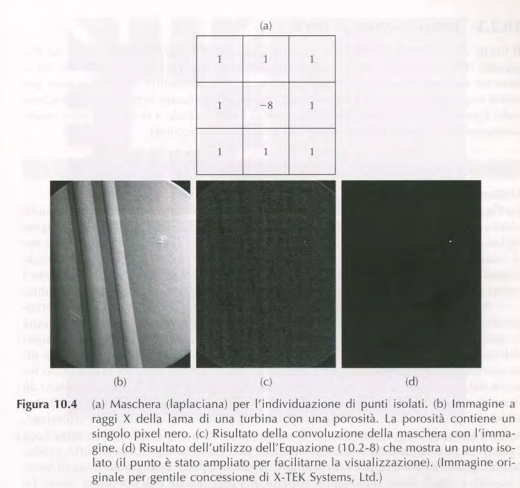
\includegraphics[width=0.8\textwidth]{Images/punti.png}
    \caption{Individuazione punti isolati}
\end{figure}
\FloatBarrier
\subsubsection{Individuazione Linee}
Sappiamo che per l'individuazione di linee potremmo aspettarci che le derivate seconde diano una risposta più forte e contestualmente producano linee più sottili rispetto alle derivate prime. Quindi, possiamo utilizzare la maschera laplaciana nella Figura 10.4a anche per l'individuazione di linee, tenendo a mente che deve essere
adeguatamente gestita la doppia risposta della derivata seconda. \\
Dato che l'immagine laplaciana contiene valori negativi, per la visualizzazione è necessaria un'operazione
di scaling (\textit{Quando una maschera di cui la somma dei coefficienti è zero è convoluta con un'immagine,
    anche i pixel nell'immagine che ne risulta avranno somma zero, caratteristica che implica l'esistenza di pixel sia negativi che positivi nel risultato. Per permetterne la visualizzazione, è necessaria un'operazione di scaling in modo tale che tutti i valori siano non negativi})
\begin{figure}[!htb]
    \centering
    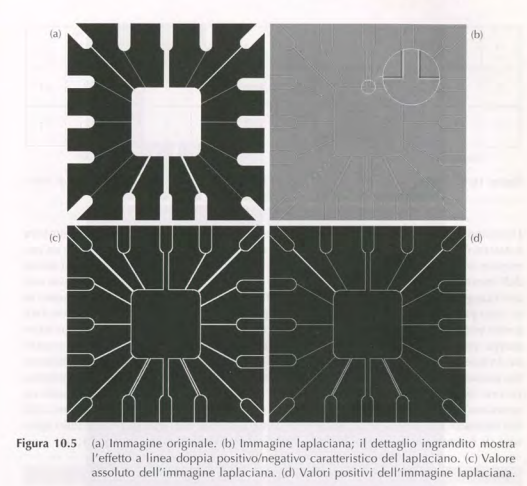
\includegraphics[width=0.8\textwidth]{Images/lapmodulo.png}
    \caption{Individuazione Linee}
\end{figure}
\FloatBarrier
L'individuatore laplaciano nella Figura 10.4a è isotropico, cioè la sua risposta è indipendente dalla direzione (rispetto alle quattro direzioni della maschera laplaciana 3 x 3: verticale, orizzontale e le due diagonali).\\Spesso, si vogliono individuare linee in direzioni specifiche.
\begin{figure}[!htb]
    \centering
    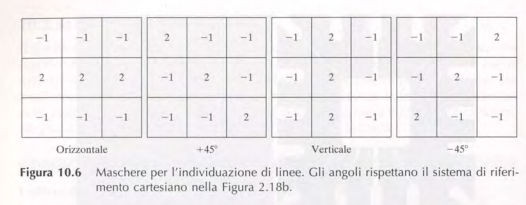
\includegraphics[width=0.8\textwidth]{Images/masch.png}
    \caption{Individuazione Linee}
\end{figure}
\FloatBarrier
\begin{figure}[!htb]
    \centering
    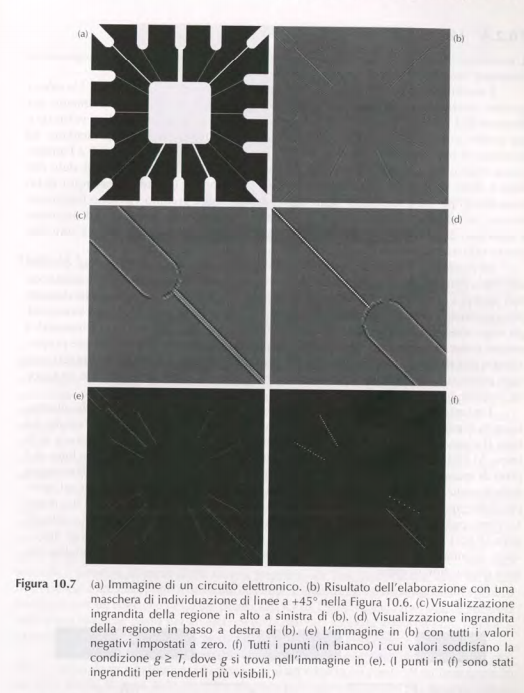
\includegraphics[width=0.6\textwidth]{Images/edgemasch.png}
    \caption{Individuazione Linee}
\end{figure}
\FloatBarrier
\newpage
\paragraph{Modelli di edge} L'individuazione degli edge è il metodo utilizzato più frequentemente per segmentare
immagini basate su bruschi (locali) cambiamenti di intensità. I modelli di edge vengono classificati secondo i loro \textbf{profili di intensità}
\begin{itemize}
    \item Un \textbf{edge a gradino} implica una transizione tra due livelli di intensità che avviene idealmente alla distanza di 1 pixel
    \item \textbf{edge a rampa}: In pratica, le immagini digitali hanno edge che sono sfocati e rumorosi, con una sfocatura determinata principalmente dalla messa a fuoco del dispositivo di acquisizione (ad esempio, lenti nel caso di immagini ottiche) e con un livello di rumore che dipenda principalmente dalle componenti elettroniche del sistema di imaging. L'ampiezza della rampa è inversamente proporzionale alla sfocatura nell'edge. In questo caso, non si ha una linea sottile (1 pixel), anzi ogni punto contenuto nella rampa è un punto di edge e un segmento di edge sarà, poi, un insieme connesso di tali punti
    \item \textbf{roof edge}, che possiede le caratteristiche illustrate nella Figura 10.8c, ed è tipicamente associato al bordo di una qualche regione
\end{itemize}
\begin{figure}[!htb]
    \centering
    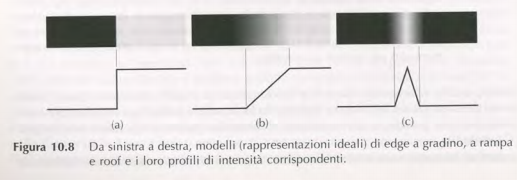
\includegraphics[width=0.8\textwidth]{Images/edgetipi-png.png}
    \caption{Tipi di edge}
\end{figure}
\FloatBarrier
La magnitudo della derivata prima può essere utilizzata per individuare la presenza di un edge in un punto di un'immagine. In maniera simile, il segno della derivata seconda può essere utilizzato per determinare se
un pixel di un edge giace sul lato scuro o chiaro di un edge.
\\Notiamo due ulteriori proprietà della derivata seconda riguardo all'edge:
\begin{itemize}
    \item esso produce due valori per ogni edge in un'immagine (caratteristica negativa)
    \item lo zero crossing può essere utilizzato per localizzare i centri di un edge
\end{itemize}
\begin{figure}[!htb]
    \centering
    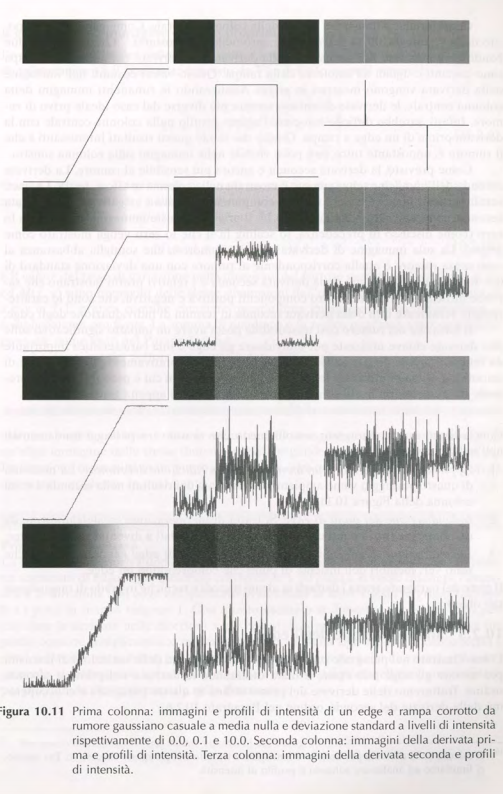
\includegraphics[width=0.7\textwidth]{Images/derrumore.png}
    \caption{Edge rumorosi}
\end{figure}
\FloatBarrier
Si deve applicare reiterativamente un operatore di smoothing prima di utilizzare le derivate in applicazioni in cui è probabile che sia presente del rumore.
\\\textbf{3 PUNTI FONDAMENTALI}:
\begin{enumerate}
    \item Applicare lo smoothing a un'immagine per la riduzione del rumore
    \item Individuazione dei punti di edge. Si tratta di un'operazione locale che estrae da un'immagine tutti i punti che sono potenziali candidati a diventare punti di edge.
    \item Localizzazione di edge. Si selezionano tra i punti di edge candidati i punti che sono veri membri dell'insieme di punti che comprendono un edge.
\end{enumerate}
\subsubsection{Individuazione degli edge}
L'individuazione delle variazioni di intensità per trovare gli edge può essere attuata utilizzando le derivate del primo e secondo ordine.
\paragraph{Gradiente e proprietà}
Lo strumento adatto per definire l'intensità e la direzione dell'edge nella posizione $(x, y)$
di un'immagine $f$ è il gradiente, denotato da $f$ e definito come il vettore:
$$\nabla f(x,y) = \begin{bmatrix}
        g_x \\
        g_y
    \end{bmatrix} = \begin{bmatrix}
        {f_{parz}'(x)} \\
        {f_{parz}'(y)}
    \end{bmatrix}
$$
Questo vettore ha l'importante proprietà geometrica di puntare nella direzione della maggiore variazione di $f $ nella posizione $(x, y)$.
La magnitudo (lunghezza) del vettore $\nabla f(x,y)$, denotato con $M(x, y)$, dove $M(x, y)=\sqrt{g_x^2+g_y^2}$ è il valore del tasso di variazione nella direzione del vettore gradiente. Un metodo spesso utilizzato (a causa dell'elevato costo computazionale nell'elevamento a potenza ed estrazione di radice) è quello di approssimare la magnitudo del gradiente tramite valori assoluti: $M(x, y)=|g_x|+|g_y|$. Questa equazione è computazionalmente più efficiente e preserva le variazioni relative tra i livelli di intensità. Il prezzo da pagare per questo vantaggio è che i filtri che ne risultano non saranno isotropici (invarianti per rotazione).
\\\textit{Si dimostra che un metodo per calcolare le derivate nelle direzioni x e y che utilizza un intorno 3 x 3 centrato su un punto consiste semplicemente nel sottrarre ai pixel nella riga superiore dell'intorno i
    pixel nella riga più in basso per ottenere la derivata parziale nella direzione x. Analogamente, si sottraggono i pixel nella colonna a sinistra dai pixel nella colonna a destra per ottenere la derivata parziale nella direzione y.}
\textbf{L'edge nel punto è ortogonale al vettore gradiente in quel punto}.
\\Ottenere il gradiente di un'immagine richiede il calcolo delle derivate parziali per ogni pixel nell'immagine. Avendo a che fare con quantità digitali, si richiede, quindi, un'approssimazione digitale delle derivate parziali in un intorno del punto.
\begin{figure}[!htb]
    \centering
    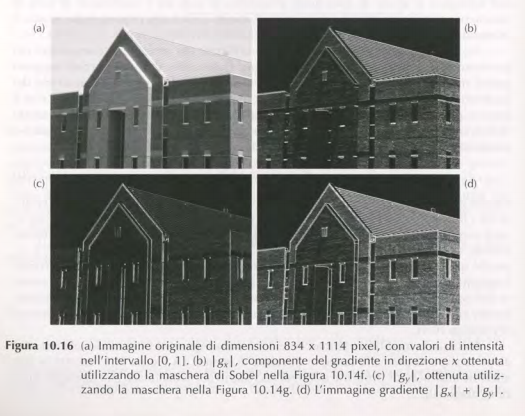
\includegraphics[width=0.8\textwidth]{Images/grad2.png}
    \caption{Gradiente}
\end{figure}
\FloatBarrier
\paragraph{Combinazione del gradiente con il thresholding}
L'individuazione degli edge può essere fatta in maniera più selettiva tramite un processo di smoothing dell'immagine da attuarsi preliminarmente al calcolo del gradiente. Un altro approccio per il raggiungimento dello
stesso obiettivo è applicare il thresholding all'immagine gradiente. Quando si vuole evidenziare sia gli edge principali che mantenere il più alto grado possibile di connettività, è pratica comune utilizzare sia lo smoothing che il thresholding.
\begin{figure}[!htb]
    \centering
    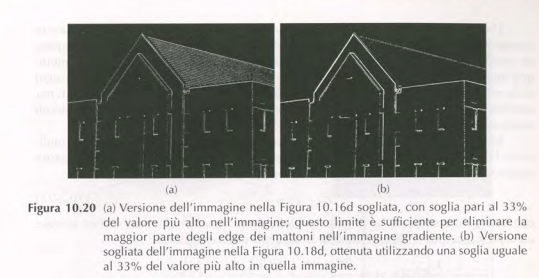
\includegraphics[width=1\textwidth]{Images/edgeT.png}
    \caption{Thresholding dopo gradiente (e media)}
\end{figure}
\FloatBarrier
\end{document}